
\section{Running \iscam; input files \& command line options}
\begin{multicols}{2}


There are three required input files for \iscam: the \verb"iscam.dat" file, the \verb"datafile", and the \verb"controlfile".  By default when \iscam runs, the first file it looks for is the \verb"iscam.dat" file, unless otherwise specified by using the command line option \verb"-ind".  The following subsections explains the details of each of the data files.


%%%%%%%%%%%%%%%%%%%%%%%%%%%%%%%%%%%%%%%%%%%
\subsection{The \texttt{iscam.dat} file}
What is required in the \verb"iscam.dat" file is just the name of the data file and the control file, in that order.  An example is given below for the \texttt{PHake2010.dat} and \texttt{Phake2010.ctl} data and control files.
\begin{verbatim}
PHake2010.dat		#Data file name
PHake2010.ctl		#Control file name
\end{verbatim}
Note that it is necessary to have the \verb"*.dat", and \verb"*.ctl" extensions, as \iscam\ will read in the entire filename including the extension.  Also note that the \verb"#" symbol acts as a comment line, and \iscam\ will ignore the contents of the remaining line when reading in data.

%%%%%%%%%%%%%%%%%%%%%%%%%%%%%%%%%%%%%%%%%%%
\subsection{The data file}
\emph{The data file and how it is set up is very important in ensuring that \iscam\ works correctly.}  In this section I have broken down the description of the data file into several blocks that deal with model dimensions, age-schedule information, removal data from each commercial and sampling gears, relative abundance information that may come from one or all of the gears,  a description of the age composition, and finally empirical weight-at-age data.  There are some data elements that are \emph{mandatory} (e.g., dimensions, age-schedule information, removals for each gear) and some optional data.  For example it is not necessary to have relative abundance information for each of the gear-type each year, or even any information on relative abundance.  Nor is it necessary to have age-composition each and every year for every gear type; in fact, it's not necessary to have any age-composition data, but in such cases selectivity parameters will have to be fixed.


The data file is composed of several required sections (required in the sense that they must be defined, but do not necessarily have to have data).  The first of these required sections is the model dimensions.  Below is an example where the model starts in 1977 and the last year is 2009, the youngest age-group is 1 years old, and the oldest age-group is 15 years old and older (i.e., a plus group).  The total number of unique gears (including gear that samples fish in surveys is two, and last line is an integer vector that specifies if the gear is a fishery, or a survey (using 1 or 0, respectively).  For each gear you must specify 1 (a commercial fishery) or 0 (a fisheries independent survey).  Again the \verb"#" is a comment character and \iscam\ will ignore the contents after this character.  The following is an example of the model dimensions section:
\begin{verbatim}
##________________________
##____Model Dimensions____
1977		#first year of data
2009		#last year of data
1			#age of youngest age class
15			#age of plus group
2			#number of gears (ngear)
## flags for gears 
## fishery (1) or 
## survey (0) in ngears
1	0
##________________________
\end{verbatim}

The next required section is the age-schedule information pertaining to natural mortality, growth and maturity-at-age. For now, natural mortality is assumed to be age-independent.
\begin{verbatim}
## ________________________
## ___Age-schedules info___
#natural mortality rate (m)
0.23
#growth parameters (linf,k,to)
52, 0.32, 0
#length-weight allometry (a,b)
5e-6, 3.0
#maturity at age (am=log(3)/k) 
#& gm=std for logistic
3.45, 0.35
## ________________________
\end{verbatim}

Next is the time series data for the historical catch by year, fishery(ies) and survey(s).  Note that it is assumed that catch exists for each year that is specified in the model dimensions section (e.g., 1977-2009).  The first column is the year of the catch, and the subsequent columns are catch (in weight) for each fishery or survey.  Years where there are no catches (or no fishery) should be replaced by a 0.  In cases where surveys did not exist, or there were no removals (e.g., an acoustic survey), specify a zero catch for each year (row).  
\begin{verbatim}
## ________________________
#Time series data
#Observed catch 
#(1977-2009, 1,000,000 metric t)
#yr	commercial survey
1977 0.132693 0
1978 0.103639 0
1979 0.137115 0
...  omitted data for space
2008 0.321546 0
2009 0.176671 0
## ________________________
\end{verbatim}

The next section pertains to the relative abundance index, where first the number (\texttt{nit}) specified the number of independent surveys, and the next row specifies the number of observations (\texttt{nit\_nobs} ,or rows of data for each survey).  The first column is an integer vector that is used to index the survey year, the second column is the actual survey abundance index, and the third column is the gear index associated with this gear.  The fourth column is the relative weight that should be used for the index.  For example, setting wt=0 for a given year will result in omitting the data, or setting wt=2 would imply that the CV is one half of the other values.  The last column specifies the fraction of total mortality that has occurred when the survey was conducted (e.g., if the survey is conducted half way through the year then 0.5 implies that 1/2 of $Z_{t,a}$ has occurred when the survey was conducted).
\begin{verbatim}
## ________________________
#Relative Abundance index from 
#independent survey (it) 1970-2008
#nit
1
#nit_nobs
13
#iyr    it gear wt survey timing
1977 1.915  2  1   0.5
1980 2.115  2  1   0.5
1983 1.647  2  1   0.5
1986 2.857  2  1   0.5
...omitted data for space
2007 0.879  2  2   0.5
2009 1.460  2  0   0.5
## ________________________
\end{verbatim}

For age-composition information, a 3 dimensional ragged array is used to store the information by gear-type (matrix), by year (rows of each matrix) and by age (columns of each matrix).  An example of the age composition data is shown in Table \ref{T1} on page \pageref{T1}.  

First you must specify the number of gears for which age-composition data exists.  If there are no data, then set this to 0. On  the next line you must specify the number of years of age-composition data there are for each gear type.  Next, for each gear type for which age-composition data is available, you must specify the first age-class of the data, and on the next row specify the oldest age-class of the data.  In the example on page \pageref{T1}, there are two gears, the first gear has 33 years of observations, and the second gear has 13 years of observations.  Each gear has the youngest age-class at 2 years and the oldest age-class at 15 years.  This means there are 14 columns of age-compositions for each gear type. 

\iscam\ treats the age-composition data as a ragged object to avoid having to read in years of missing age-composition data.  The year and gear indexes in the first two columns are used to extract predicted age-proportions to be used in the statistical comparison (negative loglikelihoods).

The first two columns of the age-composition data refer to the year and gear type from which the data were obtained.  So in the example on the next page, the first 33 rows of the matrix (some of which is missing so it could fit on the page) corresponds to the years 1977-2009 for gear type 1, and from 1977 to 2009 every 2-3 years for gear type 2.  At present \iscam\ weights each row for each gear type equally, future versions of \iscam\ will probably have a third column here where relative weights based on effective samples sizes can be specified for each observed age-composition data.

\emph{Empirical weight-at-age} data can be optionally specified immediately following the age-composition data.  By default, \iscam\ first constructs the observed weight-at-age data based on the age-schedule information specified earlier in the data file.  If there is a partial or complete set of empirical weight-at-age data available, then the default weights-at-age are overwritten for the years in which empirical data are available.    First you must specify the number of years of observed weight-at-age data as this dimensions the matrix to read in the data.  Following is a matrix where the first column specifies the corresponding year the data were collected, and for each age class defined in the model dimensions (youngest age class to plus group age class), the observed mean weights at age must be specified.  Note that the units must be in kilograms so that unit consistency in the conversion from numbers-at-age to weight-at-age can be maintained.
\begin{footnotesize}
\begin{verbatim}
#n_wt_obs
5
#Empirical mean weight-at-age in kilograms 
#A$yr  V1   V2   V3   V4   V5   V6   V7   V8   V9
1951 0.04 0.08 0.11 0.13 0.15 0.17 0.20 0.18 0.18
1952 0.04 0.08 0.11 0.13 0.15 0.17 0.16 0.17 0.18
1953 0.03 0.07 0.09 0.12 0.14 0.15 0.13 0.17 0.18
1954 0.04 0.08 0.10 0.12 0.15 0.17 0.17 0.18 0.18
1955 0.04 0.08 0.10 0.12 0.14 0.17 0.17 0.17 0.18
\end{verbatim}
\end{footnotesize}


The last component of the data file is an end of file ``eof'' marker, which is set to 999.  This is the last number read in from the datafile and \iscam\ checks to ensure it is 999.  If there is an error reading the datafile, \iscam\ will break and report that there was an error reading the data.


\begin{verbatim}
## ________________________
#eof
999
## ________________________
\end{verbatim}

\end{multicols}
%\begin{minipage}[b]{\linewidth}
%\centering
\begin{landscape}
\begin{table}
\caption{Example of age composition data in the data file.}\label{T1}
\begin{footnotesize}
\begin{verbatim}
#Age composition data by year, gear (ages 2-15+)
#na_gears
2
#na_nobs
33	13
#a_sage
2	2
#a_page
15	15
#yr 	gear       V1       V2       V3       V4       V5       V6       V7       V8       V9      V10      V11      V12      V13      V14
1977    1 0.091087 0.039290 0.208628 0.028500 0.053160 0.211179 0.078270 0.079949 0.063640 0.058483 0.043761 0.029639 0.007592 0.006823
1978    1 0.022968 0.101932 0.068633 0.199094 0.033354 0.071961 0.208406 0.084622 0.072156 0.073040 0.024682 0.021006 0.013116 0.005030
1979    1 0.049457 0.089640 0.100254 0.046571 0.191908 0.071243 0.159754 0.158389 0.056370 0.037676 0.016184 0.010295 0.006469 0.005789
1980    1 0.009331 0.254593 0.042151 0.054263 0.050507 0.143816 0.065236 0.087843 0.169471 0.046122 0.037636 0.023076 0.008874 0.007079
1981    1 0.091224 0.062768 0.280898 0.012851 0.045430 0.047641 0.148751 0.062707 0.066417 0.125977 0.031183 0.012419 0.009671 0.002062
1982    1 0.181412 0.025886 0.016978 0.318964 0.032603 0.045648 0.045099 0.131034 0.027439 0.033879 0.119575 0.010972 0.006862 0.003648
1983    1 0.000322 0.327381 0.030386 0.021774 0.318861 0.034486 0.037515 0.044368 0.095257 0.024331 0.017871 0.037722 0.007340 0.002385
1984    1 0.000000 0.010415 0.546489 0.035445 0.072340 0.185115 0.023775 0.020842 0.014283 0.045333 0.009533 0.007920 0.024390 0.004121
1985    1 0.006798 0.006334 0.065169 0.607023 0.070421 0.058060 0.132423 0.011557 0.006879 0.007111 0.013539 0.002836 0.000000 0.011849
1986    1 0.111570 0.031159 0.007757 0.034088 0.485333 0.058011 0.043959 0.122124 0.022909 0.026576 0.014536 0.026627 0.004392 0.010957
1987    1 0.000000 0.264654 0.016305 0.003861 0.017893 0.540852 0.032262 0.016639 0.080708 0.003902 0.001822 0.005542 0.009811 0.005748
1988    1 0.002907 0.002881 0.325484 0.012085 0.007047 0.010794 0.464716 0.021331 0.009870 0.101698 0.001949 0.004157 0.001274 0.033806
1989    1 0.026833 0.022546 0.009612 0.452262 0.010250 0.004556 0.006132 0.394579 0.015267 0.006758 0.044542 0.000903 0.001179 0.004583
1990    1 0.048604 0.255566 0.024077 0.002273 0.251121 0.006576 0.001663 0.000990 0.323920 0.003924 0.000212 0.072414 0.000146 0.008513
1991    1 0.034754 0.176910 0.169392 0.027073 0.007271 0.316749 0.012094 0.001274 0.001349 0.206127 0.003853 0.000000 0.036791 0.006363
1992    1 0.035191 0.044184 0.126581 0.177710 0.021788 0.007533 0.344623 0.006212 0.001264 0.003920 0.198907 0.004982 0.000449 0.026655
1993    1 0.007327 0.219650 0.032109 0.141618 0.169717 0.014288 0.007544 0.287667 0.008052 0.001062 0.000425 0.104591 0.000492 0.005457
1994    1 0.000419 0.033794 0.194593 0.013819 0.121828 0.200067 0.013059 0.004773 0.307047 0.002355 0.004118 0.000280 0.096116 0.007732
1995    1 0.015172 0.001676 0.067824 0.247580 0.011946 0.076025 0.204514 0.017753 0.003065 0.259156 0.002369 0.003815 0.000000 0.089107
...	some missing data removed here to fit on page.
2005    1 0.008720 0.004799 0.070427 0.055023 0.684012 0.084118 0.021823 0.028355 0.019809 0.010432 0.008069 0.002582 0.000360 0.001470
2006    1 0.016047 0.109332 0.016100 0.086023 0.047267 0.606611 0.050565 0.017944 0.019738 0.012433 0.009263 0.004693 0.001532 0.002454
2007    1 0.135250 0.030604 0.145496 0.015585 0.070675 0.041936 0.441809 0.059055 0.018388 0.018549 0.012342 0.004254 0.004551 0.001507
2008    1 0.086419 0.307710 0.023174 0.134343 0.009449 0.035456 0.033322 0.305151 0.032058 0.010867 0.008882 0.005414 0.003330 0.004426
2009    1 0.007237 0.201241 0.298293 0.044466 0.140682 0.014182 0.025967 0.022153 0.193496 0.036166 0.005012 0.004290 0.003855 0.002961
1977    2 0.054308 0.051673 0.322415 0.029524 0.041387 0.358094 0.049372 0.036486 0.020920 0.019594 0.010201 0.003792 0.000997 0.001237
1980    2 0.004557 0.555127 0.053761 0.032569 0.026590 0.117668 0.043603 0.093838 0.037630 0.022180 0.003734 0.006424 0.001338 0.000983
1983    2 0.000265 0.785009 0.026011 0.007869 0.103384 0.016545 0.011402 0.008131 0.022356 0.005273 0.006223 0.006489 0.001042 0.000000
1986    2 0.604601 0.015879 0.002792 0.019748 0.266035 0.028628 0.022778 0.029920 0.003627 0.003812 0.000276 0.001440 0.000463 0.000000
1989    2 0.169990 0.058515 0.012874 0.526835 0.011735 0.004161 0.007554 0.179632 0.009473 0.000722 0.017782 0.000000 0.000000 0.000726
1992    2 0.089253 0.011915 0.069071 0.176823 0.021856 0.008862 0.432238 0.013086 0.007872 0.003964 0.149487 0.007606 0.000000 0.007967
1995    2 0.324964 0.043475 0.012039 0.212541 0.009810 0.032765 0.148871 0.002177 0.000000 0.158452 0.000354 0.006429 0.000000 0.048122
1998    2 0.168351 0.187074 0.157169 0.195749 0.014026 0.055093 0.087607 0.010731 0.015903 0.048868 0.003121 0.001999 0.042448 0.011861
2001    2 0.709921 0.089531 0.052761 0.056572 0.026180 0.026069 0.014190 0.008255 0.005804 0.002446 0.002162 0.004212 0.000400 0.001496
2003    2 0.029781 0.025334 0.640666 0.109500 0.027623 0.060058 0.039723 0.021949 0.022287 0.007181 0.004232 0.004367 0.003083 0.004214
2005    2 0.239916 0.024324 0.072095 0.051813 0.482518 0.052666 0.017966 0.024352 0.013884 0.011229 0.004744 0.002436 0.000323 0.001734
2007    2 0.428146 0.024375 0.101876 0.011527 0.041221 0.026044 0.289941 0.030229 0.013473 0.013191 0.007185 0.006086 0.002778 0.003928
2009    2 0.001881 0.229516 0.423131 0.024861 0.091878 0.007856 0.018074 0.024434 0.128613 0.029027 0.009417 0.005566 0.005402 0.000343
\end{verbatim}
\end{footnotesize}
\end{table}
\end{landscape}




%%%%%%%%%%%%%%%%%%%%%%%%%%%%%%%%%%%%%%%%%%%
\begin{multicols}{2}
\subsection{The control file (still under development)}
The first section of the control file pertains to the leading parameter vector which is summarized in Table \ref{Table.parameter.controls}.  For now, there are 6 leading parameters for which the initial values (ival) lower (lb) and upper bounds (ub) and estimation phase must be specified.  Each of these parameters also have parameters for the corresponding prior distributions defined by the prior\_type, and parameters p1 and p2.

\begin{tablehere}\caption{Controls for estimated parameters in the control file.}\label{Table.parameter.controls}
\begin{tiny}
\begin{verbatim}
## ____________________________________________________________________________ ##
##                            PACIFIC HAKE CONTROLS
## ___________________CONTROLS FOR ESTIMATED PARAMETERS________________________ ##
##  Prior descriptions:
##                      -0 uniform (0,0)
##                      -1 normal (p1=mu,p2=sig)
##                      -2 lognormal (p1=log(mu),p2=sig)
##                      -3 beta (p1=alpha,p2=beta)
##                      -4 gamma(p1=alpha,p2=beta)
## ____________________________________________________________________________ ##
6   ## npar
##  ival        lb      ub      phz     prior    p1      p2      parameter name
## ____________________________________________________________________________ ##
    1.6         -5.0    15       4       1       0.9     0.5     #log_ro/msy 
    0.65        0.2     1.0      4       3       3       2       #steepness/fmsy
    -1.469      -5.0    0.0      2       1       -1.469  0.05    #log.m
    1.6         -5.0    15       1       0       -5.0    15      #log_avgrec
    0.2         0.001   0.999    3       3       3.75    12      #rho
    1.25        0.01    500      3       4       1.01    1.01    #kappa (precision)
## ____________________________________________________________________________ ##
\end{verbatim}
\end{tiny}
\end{tablehere}
%	%\end{multicols}
%	
%	%\begin{table*}[h]
%	\begin{tablehere}
%	\caption{Controls for estimated parameters in the control file.}
%	\begin{center}
%	\begin{tiny}
%	\begin{tabular}{llllclll}
%	6 & \#npar \\
%	\hline
%	\#ival & lb & ub & phz & prior\_type & p1 & p2 & parameter name\\
%	\hline
%	1.2 & -5.0 & 15.0 & 3 & 0 & 0 & 0 & \#log\_ro or log\_msy\\
%	0.75 & 0.2 & 1.0 & 3 & 3 & 1.01 & 1.01 & \#steepness or log\_fmsy\\
%	-1.5 & -5.0 & 2.0 & -1 & 0 & 0 & 0 & \#log\_m\\
%	1.0 & -5.0 & 15.0 & 1 & 0 & 0 & 0 & \#log\_avg\_rec\\
%	0.2 & 0.001 & 0.999 & -1 & 3 & 30 & 30 & \#rho\\
%	1.25 & 0.01 & 500.0 & -1 & 4 & 1.01 & 1.01 & \#kappa (total precision)\\
%	\hline
%	\end{tabular}
%	\end{tiny}
%	\end{center}
%	\label{Table.parameter.controls}
%	\end{tablehere}
%	
%	%\begin{multicols}{2}
\subsubsection{Prior type distributions}
As of now there are 5 different prior types that can be specified and these are given by the integer values 0--4.  The following list describes the prior types and the parameter values for the distributions:
\begin{description}
\item[0] A uniform prior between lb and up. 
\item[1] A normal prior p1 = mean, and p2 = standard deviation
\item[2] A lognormal prior p1 = log(mean), and p2 = log standard deviation
\item[3] A beta prior p1 = alpha, and p2 = beta with lb and ub transformed to a 0-1 scale.
\item[4] A gamma prior with p1=alpha and p2=beta
\end{description}

\begin{figurehere}
	% Requires \usepackage{graphicx}\
	\centering
	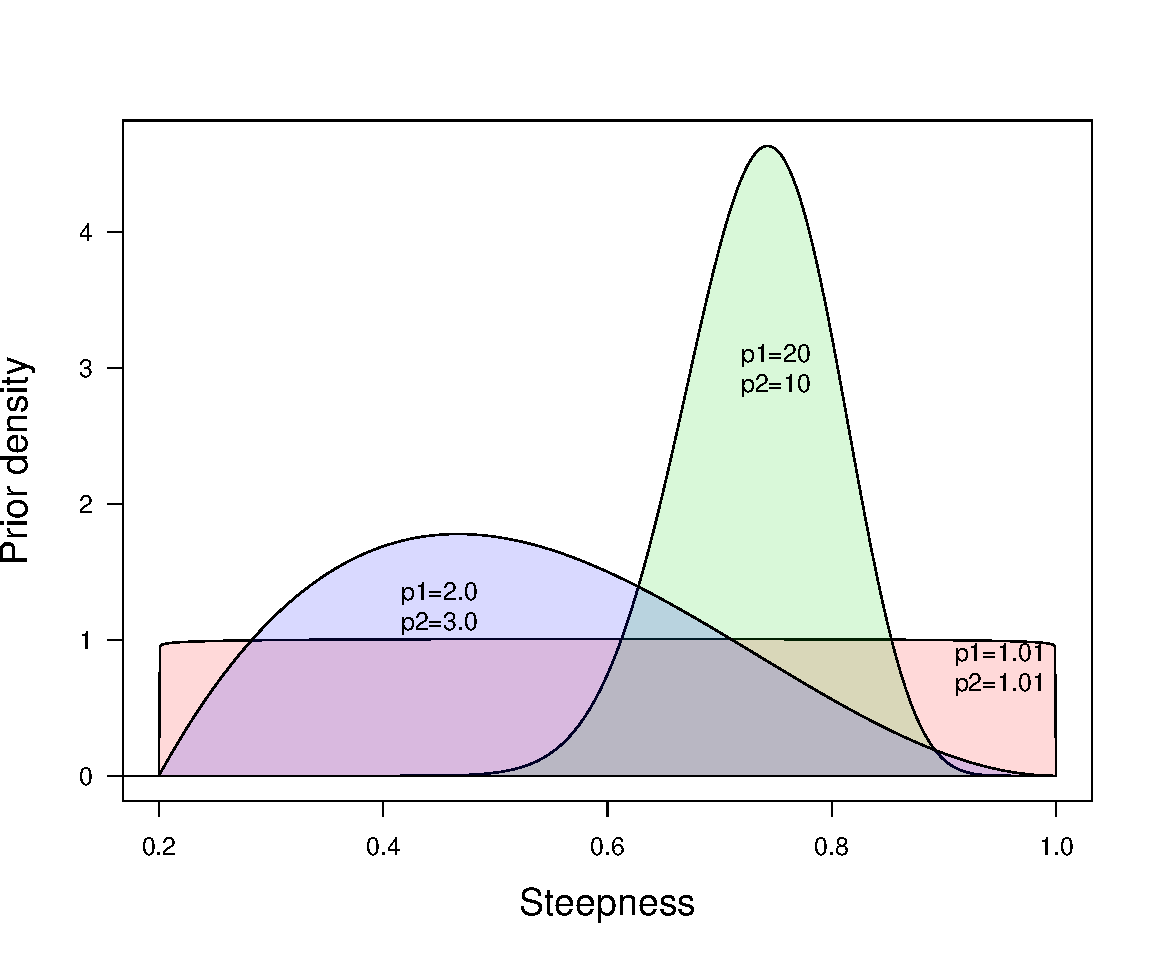
\includegraphics[width=\columnwidth]{iscamFigs/betaPriors.pdf}\\
	\caption{Three alternative beta prior distributions with corresponding values of p1 and p2 specified on the distribution.  Note that specifying values of 1.01 results in a more or less uniform prior distribution for steepness in the Beverton-Holt stock recruitment model.}\label{label}
\end{figurehere}

\subsubsection{Selectivity controls}
The next table of numbers in the control file contains the options for selectivities for each of the gear types (both fisheries and surveys).  Currently there are 6 options implemented for selectivities in \iscam\, and the details of each are explained further in the model documentation section (see page \pageref{ModelDocSelectivity}).  The following is an excerpt from the Pacific hake control file with selectivities defined for two gears:

\begin{tiny}
\begin{verbatim}
## _________________________SELECTIVITY PARAMETERS_____________________________ ##
## OPTIONS FOR SELECTIVITY:
##      1) logistic selectivity parameters
##      2) selectivity coefficients
##      3) a constant cubic spline with age-nodes
##      4) a time varying cubic spline with age-nodes
##      5) a time varying bicubic spline with age & year nodes.
##      6) fixed logistic (set isel_type=1, and estimation phase to -1)
## Gear 1 fishery:  Gear 2 survey
## isel_type
    5        1
## Age at 50% selectivity (logistic)
    3.5      4.0
## STD at 50% selectivity (logistic)
    1.0      0.5
## No. of age nodes for each gear (0 to ignore).
    5        5
## No. of year nodes for each gear (0 to ignore).
    11       3
## Estimation phase
    2        2
## Penalty weight for 2nd differences w=1/(2*sig^2)
    12.5     12.5
## Penalty weight for dome-shaped selectivity 1=1/(2*sig^2)
    3.125    200.0
## ____________________________________________________________________________ ##
\end{verbatim}
\end{tiny}
There are two gears specified in this case, the first gear uses the time varying bicubic spline option with 5 age nodes and 11 year nodes and is estimated in phase 2 of the parameter search routine.  The second fishery (second column) is a survey with a logistic selectivity function with initial values of 4.0 and 0.5 as the mean and standard deviation that is assumed in the first phase; in the second phase these values are then treated as estimated parameters.  The last two rows of the selectivity controls defines the penalty weights used for the selectivity ogives where the 2nd differences controls the smoothness of the curve and the dome-shaped penalty limits how much the selectivity decline with older ages (dome-shaped).  Note that these two penalties are ignored for the logistic (option 1 and option 6) forms of the selectivity curve.


\subsubsection{Priors for survey catchability}
Although the scaling parameters for surveys or relative abundance indices are not directly estimated, it is possible to specify prior distributions for the conditional maximum likelihood estimates of these parameters. Priors are specified by the following four lines in the control file, there \verb"nits" is simply the number of relative abundance indices.  In the following rows, you must specify a `0' or `1' for a uniform prior or an informative prior distribution.  Note that if there is more than 1 survey, then you'll have to specify a 0 or 1 for each of the surveys (i.e., columns for each survey).  The final two rows specify the log mean of the normal prior and the standard deviation (if they prior type is uniform you must still specify these values, however they are ignored in the objective function calculation; future versions may specify lower and upper bounds of a true uniform density).  Again, in the case of multiple surveys, you must have a mean and standard deviation specified (in columns) for each of the surveys.

\begin{tiny}
\begin{verbatim}
## ____________________________________________________________________________ ##
##                             Priors for Survey q                              ##
## ____________________________________________________________________________ ##
## nits  #number of surveys
    1
## priors 0=uniform density     1=normal density
    0
## prior log(mean);
    0
## prior sd
    1
## ____________________________________________________________________________ ##
\end{verbatim}
\end{tiny}


\subsubsection{Other miscellaneous controls}
The following is an ordered list of controls that turn various switches on and off or set up alternative structural assumptions such as Ricker recruitment or time varying natural mortality rates in \iscam.  It's also a place holder to add additional features to \iscam\ as the model continues to evolve over time. The following is an ordered list describing in more detail each of the miscellaneous controls.

\begin{enumerate}

	\item The first row of the miscellaneous controls is a flag that turns on and off the verbose output of \iscam.

	\item Switch between Beverton-Holt  recruitment \eqref{T4.12} and Ricker recruitment \eqref{T4.13}.
	
	\item The assumed standard deviation (in log space) in the observed catch in all phases except the last phase of the parameter estimation scheme.  Note that this value must be greater than 0.  Slightly larger values (say 0.05) will speed up convergence in earlier phases.
	
	\item The assumed standard deviation (in log space) in the observed catch in the last phase of the parameter estimation scheme.  Note that this value must be greater than 0.  Slightly smaller values (say 0.01) will increase precision in the estimates of F but generally slow down convergence.
		
	\item The next item is a flag to initialize the model at an unfished state in the initial year, otherwise, \iscam\ estimates the numbers at age in the first year.
	
	\item Age-composition data are pooled into plus groups if the observed proportions-at-age are less than the specified percentage (e.g., $<$1\% in the example control file below).  See description of age-cmposition data, specifically the last paragraph in section \ref{agecomps} on page \pageref{agecomps}.
	
	\item During the initial phases of the parameter estimation, a large penalty is used to regularize the estimates of the annual fishing mortality rates and then in the last phase this penalty is relaxed.  The penalty is on deviations from the average fishing mortality rate (0.20 in the example below) for all fishing fleets.  
	
	\item The assumed standard deviation (in log space) in the fishing mortality rate penalty in the initial phases.
	
	\item The assumed standard deviation (in log space) in the fishing mortality rate in the last phase, (should be a large value (e.g., 5 or greater), otherwise the penalty could reduce the true variation in the estimated $F_t$'s.
	
	\item The option to estimate changes in natural mortality rates via a random walk process is implemented by selecting a positive phase (negative values imply a constant $M$) and annual deviations in $M$ are not estimated.
	
	\item  If annual deviations in natural mortality are estimated, then the standard deviation for the normal prior for deviations in $M_t$ are specified here.
\end{enumerate}




\begin{tiny}
\begin{verbatim}
## _______________________OTHER MISCELLANEOUS CONTROLS_________________________ ##
0           ## verbose ISCAM output (0=off, 1=on).
1           ## recruitment model (1=beverton-holt, 2=ricker).
0.05        ## std in observed catches in initial phases.
0.01        ## std in observed catches in last phase.
0           ## Assume unfished in first year (0=FALSE, 1=TRUE).
0.01        ## Minimum proportion to consider in age-proportions for dmvlogistic.
0.20        ## Mean fishing mortality for regularizing the estimates of Ft.
0.01        ## std in mean fishing mortality in initial phases.
5.00        ## std in mean fishing mortality in last phase.
-1          ## phase for estimating m_deviations (use -1 to turn off mdevs).
0.1         ## std in deviations for natural mortality.
## ____________________________________________________________________________ ##

\end{verbatim}
\end{tiny}


\end{multicols}

%\begin{figure*}[b]
%	% Requires \usepackage{graphicx}
%	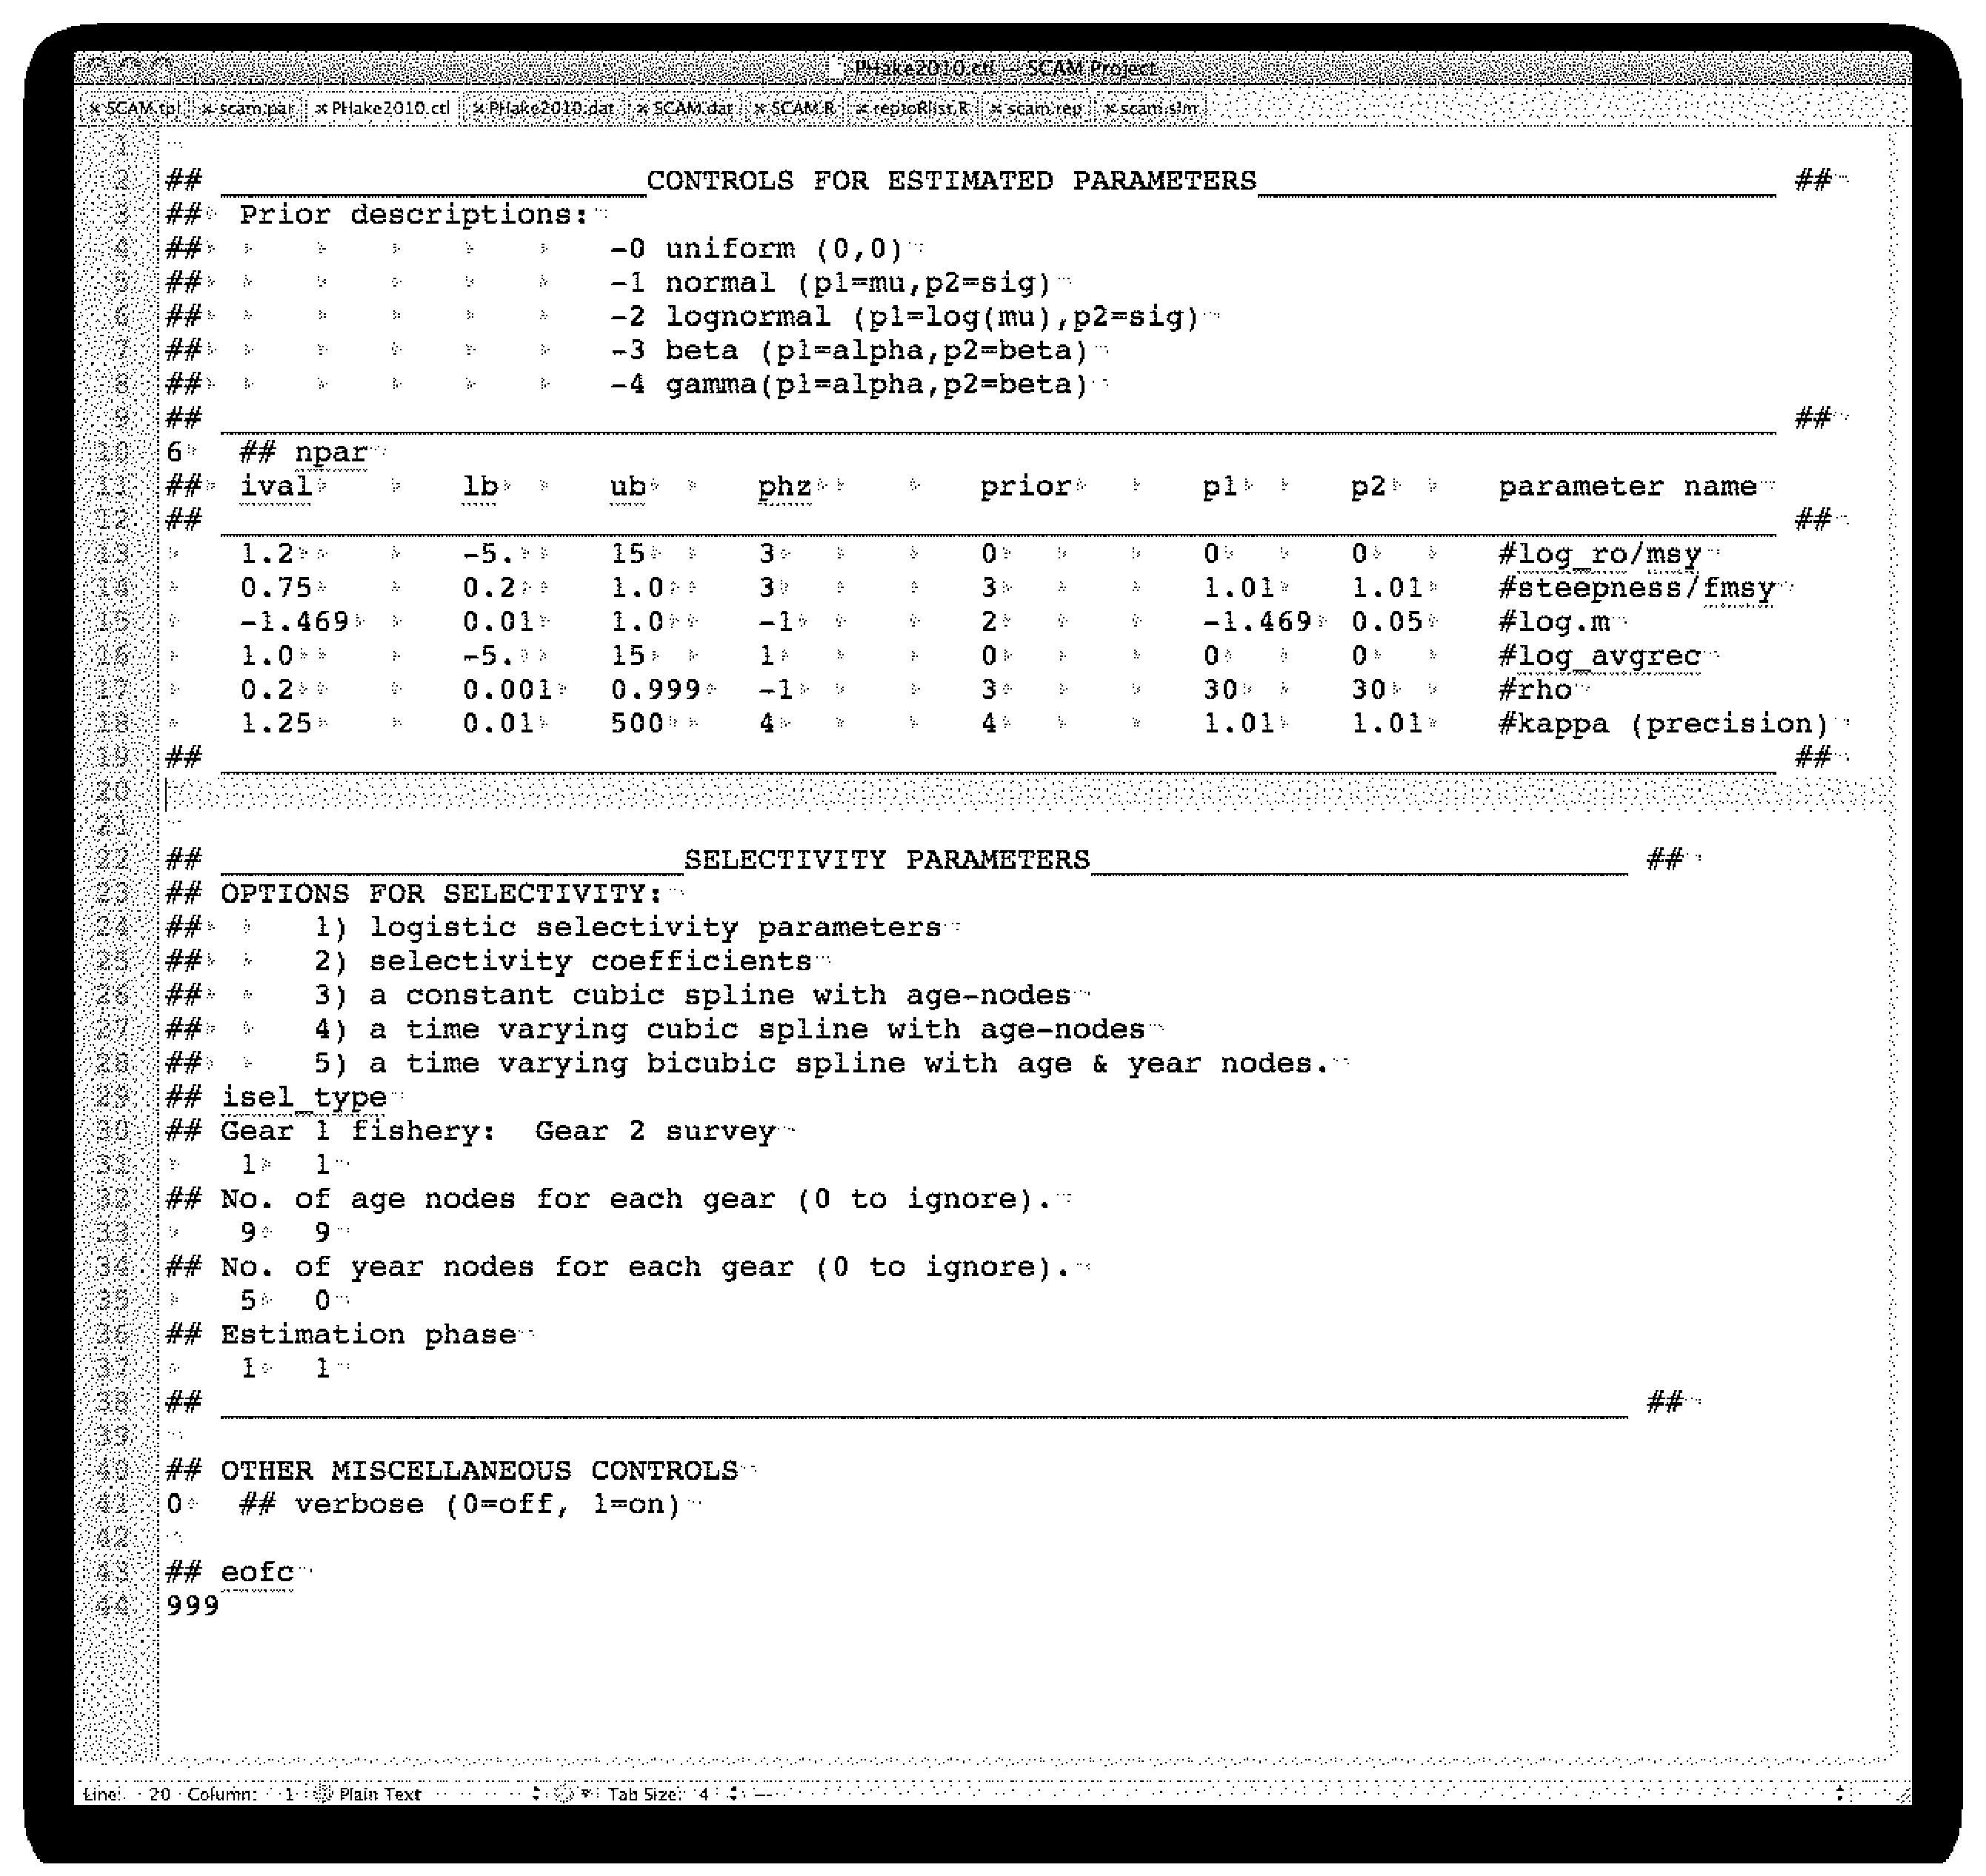
\includegraphics[width=\textwidth]{sc1.eps}\\
%	\caption{A screen shot of the example control file.}\label{Fig.control.file}
%\end{figure*}



\begin{multicols}{2}

\subsection{Command line options}
Currently there are two custom command line options available in \iscam\ in addition to the standard command line options provided by the AD Model Builder libraries (see help command line options -? for more information on the ADMB command line options). 

The custom command line options are:
\begin{description}
\item[-sim N] use this option turn the model into a simulation model, where N is the random number seed.

\item[-retro N] use the option for retrospective analysis where the last N years of data are ignored in the likelihood calculations.
\end{description}

There two random number seeds for the simulation model that the user should be aware of.  The first is if the random number seed is set to 000, then \iscam\ will actually simulate data with no errors whatsoever.  That is, the values of $\sigma$ and $\tau$ (observation error and process errors, respectively) will be set equal to 0 and the simulation model will run as a deterministic model with no observation errors in the relative abundance index or age composition data.  This option allows the user to check to ensure that the model parameters are in fact estimable with perfect information.


The second unique random seed number is 99, and this seed number is used for the simulation example in this manuscript.  It specifies a unique time-varying selectivity curve for the commercial fishery that goes from dome-shaped to asymptotic.

\subsubsection{Running the simulation model}

Again, one of the first steps in conducting any assessment should be to first run the model on simulated data with no error to be certain that the model is capable of estimating the specified model parameters.  To do so in \iscam\, the user simply needs to specify the command line option of \texttt{-sim 000}, where the `000' argument specifically instructs \iscam\ not to add any random variation to the observation or process errors.  Invoking this command line option will run \iscam\ as normal, where the data from the data file is first read into memory, then the information from the control file is then read in.  However, before proceeding straight into the non-linear parameter estimation procedure, \iscam\ first runs a simulation model based on the specified parameters listed in the control file.  This simulation model will then replace the existing data in memory with simulated data, then perform the non-linear parameter estimation procedure and attempt to estimate the model parameters.  If all is working well the estimated parameters listed in the parameter file should be very close, if not exactly, to the initial values specified in the control file.




\end{multicols}
